\documentclass[a4paper, 12pt]{article}
\usepackage[left=2cm, top=3cm, text={17cm, 24cm}]{geometry}
\usepackage{times}
\usepackage{multirow}
\usepackage[czech]{babel}
\usepackage[IL2]{fontenc}
\usepackage[ruled, czech, linesnumbered, noline, longend]{algorithm2e}
\usepackage{graphicx}
\usepackage{pdflscape}
\usepackage[unicode]{hyperref}

%%%%%%%%%%%%%%%%%%%%%%%%%%%%%%%%%%%%%%% Úvodní stránka %%%%%%%%%%%%%%%%%%%%%%%%%%%%%%%%%%%%%%%

\begin{document}
\catcode`\-=12

\begin{titlepage}
		\begin{center}
			\Huge
			\textsc{Vysoké učení technické v~Brně} \\
			\huge
			\textsc{Fakulta informačních technologií} \\
			\vspace{\stretch{0.382}}
			
\includegraphics[scale=0.9]{img/FIT_barevne_CMYK_CZ.pdf} \\
			\Huge
			Finální schéma databáze \\
			\huge
			Pekárna
			\vspace{\stretch{0.618}}
		\end{center}
		\begin{itemize}
		    \item[] \large{Daniel Fajmon - xfajmo05}
		    \item[] \large{Jakub Dunčko - xdunck01 \hfill \today}
		\end{itemize}
\end{titlepage}

%%%%%%%%%%%%%%%%%%%%%%%%%%%%%%%%%%%%%%% 0. Obsah %%%%%%%%%%%%%%%%%%%%%%%%%%%%%%%%%%%%%%%
\tableofcontents
\newpage

%%%%%%%%%%%%%%%%%%%%%%%%%%%%%%%%%%%%%%% 1. Zadání %%%%%%%%%%%%%%%%%%%%%%%%%%%%%%%%%%%%%%%
\section{Zadání}
Navrhněte jednoduchý informační systém pekárny, který bude spravovat informace o nabízených druzích pečiva jak z hlediska výroby (suroviny, náklady atd.), tak odbytu (objednávky). Pekárna zajišťuje rozvoz vlastními auty nebo si odběratelé odvoz zajišťují sami. Systém musí umožnit vedení pekárny plánovat produkci v závislosti na objednávkách, poskytovat informace pro rozvoz apod.

%%%%%%%%%%%%%%%%%%%%%%%%%%%%%%%%%%%%%%% 2. Popis systému %%%%%%%%%%%%%%%%%%%%%%%%%%%%%%%%%%%%%%%
\section{Popis systému}
Systém umožňuje zákazníkům snadné vytváření objednávek na pečivo z aktuální nabídky a získání informací o složení včetně alergenů. Zákazníci mohou volit způsob dopravy a sledovat stav své objednávky.

Ředitel výroby má přehled o počtu objednávek, plánuje objednávání surovin a pečiva a přiděluje firemní auta šoférům. Dále má možnost zobrazit náklady za palivo za aktuální den. Pekaři a šoféři mohou upravovat stav objednávek (zpracovává se, připravena k vyzvednutí, doručena).

Systém také ukládá informace o zaměstnancích a zákaznících a umožňuje jejich úpravu nebo smazání.

%%%%%%%%%%%%%%%%%%%%%%%%%%%%%%%%%%%%%%% 3. Pojmy %%%%%%%%%%%%%%%%%%%%%%%%%%%%%%%%%%%%%%%
\section{Pojmy}
\begin{description}
   \item Jako \textbf{generalizaci} jsme použili entity pekaře a šoféra, kteří dědí vlastnosti zaměstnance.
   \item \textbf{Číslo účtu} si u zákazníka pamatujeme z důvodu dalších možných objednávek a tím ulehčili práci se systémem a urychlením zpracování.
   \item \textbf{Nabídka} zahrnuje všechny druhy pečiva, které je možné upéct ze surovin na skladě nebo
možné doobjednat podle zákazníkových potřeb.
    \item \textbf{Náklady za cestu} jsou spotřebované pohonné hmoty za konkrétní rozvoz.
    \item \textbf{Spravovat osobní informace} je případ, kdy zaměstnanec může měnit svoje osobní
informace, ale není schopen měnit informace ostatních zaměstnanců.
    \item \textbf{Alergeny} zpracováváme podle tabulky hlavních potravinových alergenů a pečivu se přidávají
pouze čísla alergenu.
    \item \textbf{Spravovat informace o zaměstnancích} - pouze ředitel je schopen měnit datum nástupu zaměstnance a jeho výši mzdy. 
\end{description}

%%%%%%%%%%%%%%%%%%%%%%%%%%%%%%%%%%%%%%% 4. ER Diagram %%%%%%%%%%%%%%%%%%%%%%%%%%%%%%%%%%%%
\section{Entity Relationship Diagram}
\begin{center}
    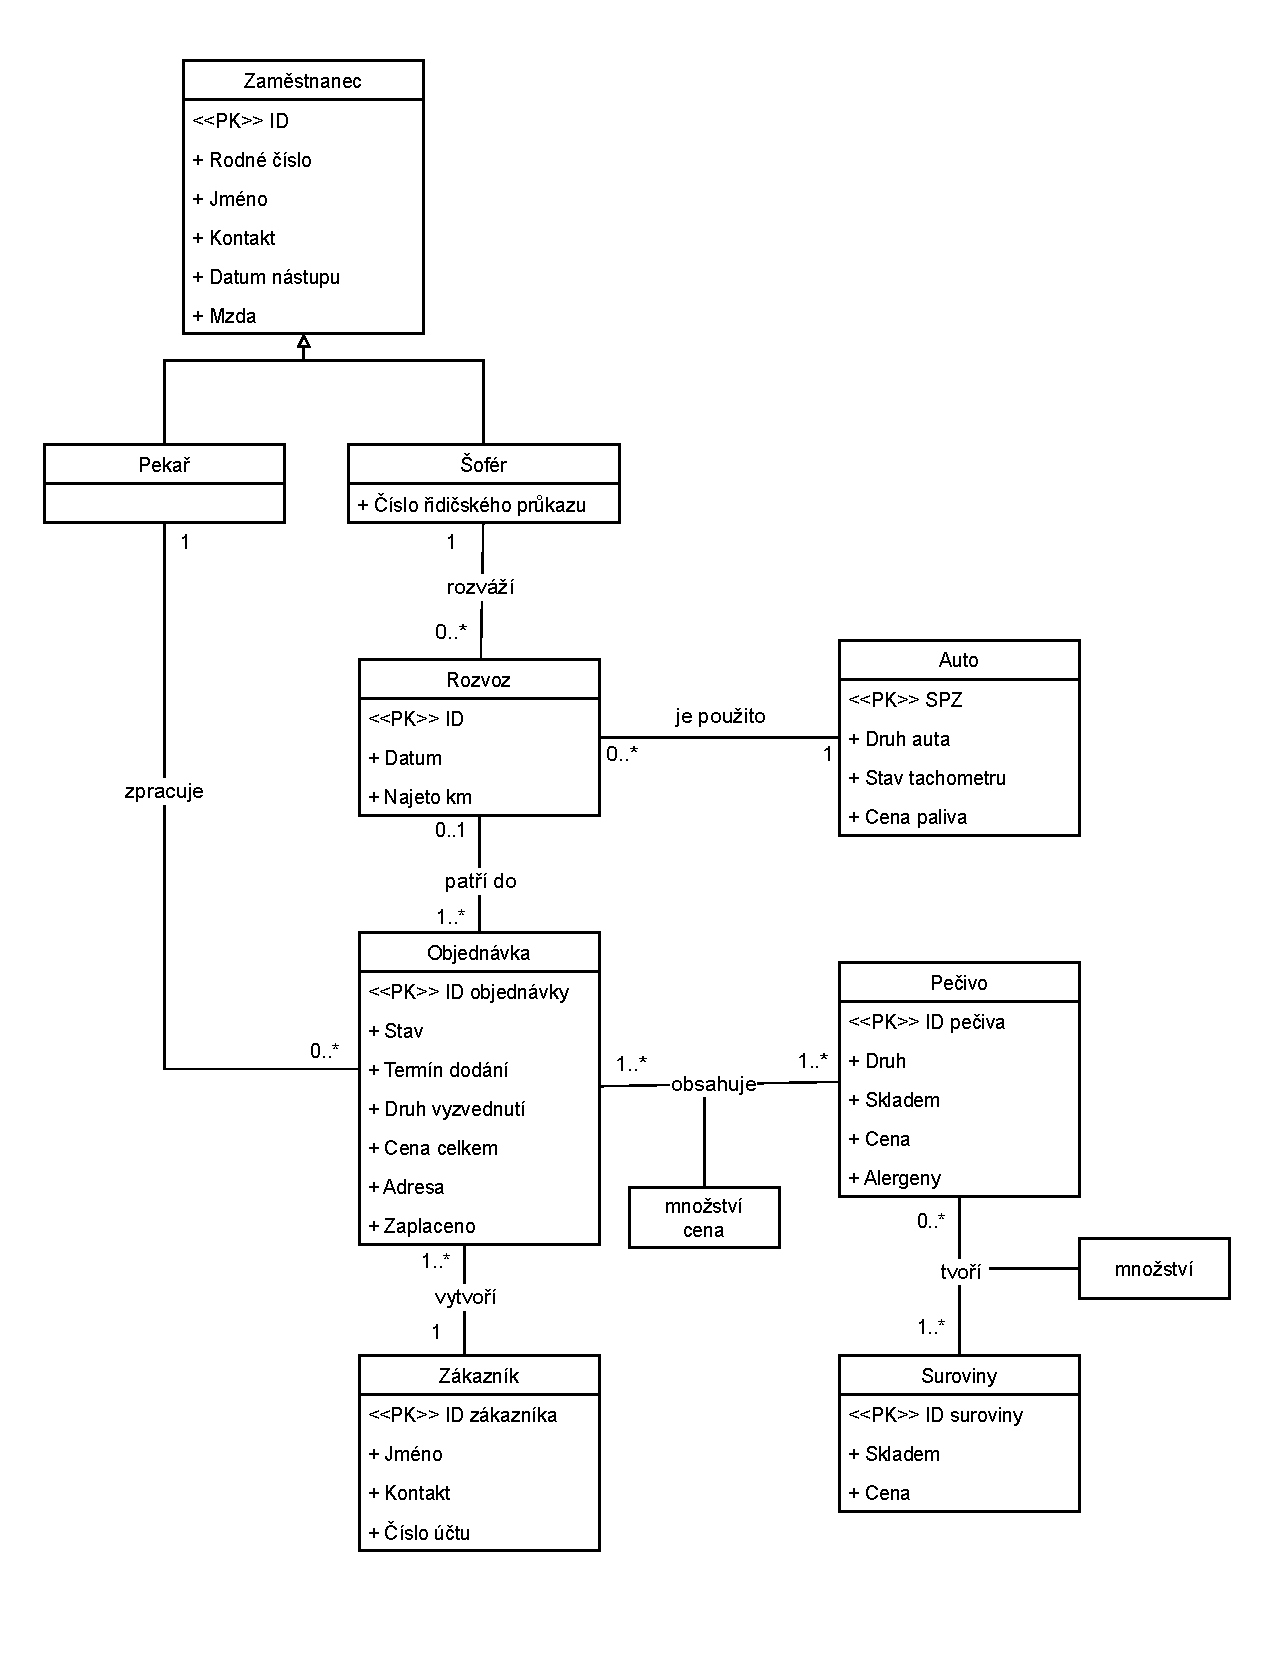
\includegraphics[scale=0.75]{img/erd.pdf}
\end{center}

%%%%%%%%%%%%%%%%%%%%%%%%%%%%%%%%%%%%%%% 5. UML %%%%%%%%%%%%%%%%%%%%%%%%%%%%%%%%%%%%%%%%%%%
\section{Use Case Diagram}
\begin{center}
    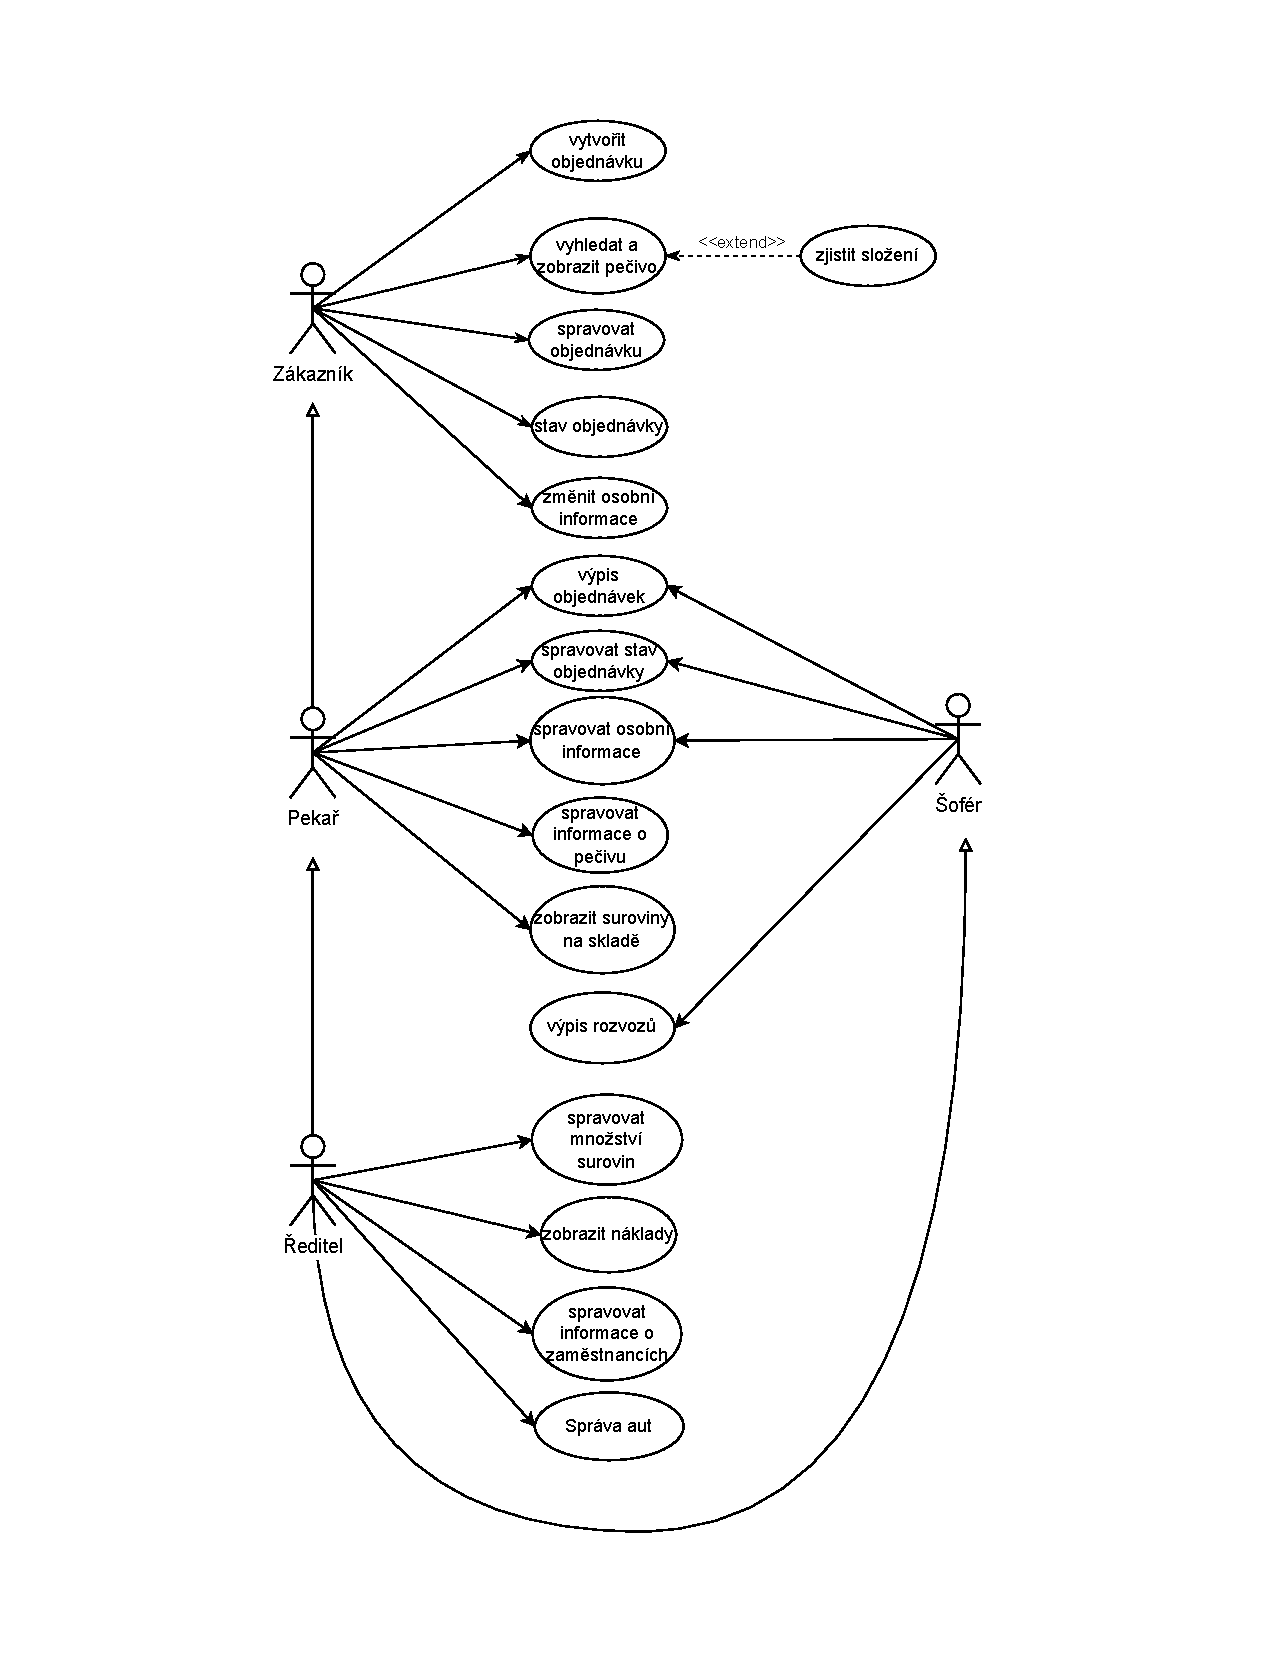
\includegraphics[scale=0.75]{img/uml.pdf}
\end{center}

%%%%%%%%%%%%%%%%%%%%%%%%%%%%%%%%%%%%%%% 6. Generalizace %%%%%%%%%%%%%%%%%%%%%%%%%%%%%%%%%%%
\section{Generalizace}
Jako generalizaci jsme využili pekaře a šoféra, kteří dědí z tabulky zaměstnanec. V databázi jsme to implementovali tabulku zaměstnanec, ze které dědí ID.

%%%%%%%%%%%%%%%%%%%%%%%%%%%%%%%%%%%%%%% 7. Implementace %%%%%%%%%%%%%%%%%%%%%%%%%%%%%%%%%%%
\section{Implementace}
\subsection{Drop table}
Smazání duplicitních tabulek v případě, že tabulky se stejným názvem již existují. Bez tohoto by nebylo možné skript pouštět opakovaně.

\subsection{Create table, insert, check}
Vytvoření tabulek s atributy a kontrolami nad daty. Nastavení sdílených klíčů. Následně vložení dat.

\subsection{Select}
Vytvoření tabulek, které mohou uživatelé databáze použít.
\begin{itemize}
    \item[1] Informace o zákazníkovi a objednávce
    \item[2] Informace o řidiči
    \item[3] Informace pro řidiče kam a komu doručit objednávku
    \item[4] Počet objednávek podle druhu vyzvednutí
    \item[5] Kolik pečiva je třeba vypéct na objednávku
    \item[6] Výpis objednávek, které lze vyzvednout
    \item[7] Výpis kolik je potřeba materiálu na všechny aktuální objednávky
\end{itemize}

\subsection{Trigger}
Za úkol bylo vytvořit 2 triggery. My jsme vytvořily:
\begin{itemize}
    \item[1] {Zrušení objednávky podle datumu}
    \item[2] {Zrušení objednávky podle množství pečiva}
\end{itemize}
Náš první trigger kontroluje, že objednávka má termín objednání menší jak termín dodání. V opačném případě dojde k erroru a vypíše se "\texttt{Neplatný termín dodání. Dodání musí být v budoucnosti.}".
Druhý trigger kontroluje, že objednávka obsahuje počet pečiva větší jak 0, jinak dojde k chybové hlášce "\texttt{Počet pečiva na objednávce musí být větší jak 0.}".

\subsection{Explain plan}
EXPLAIN PLAN je příkaz, který poskytuje informace o plánu dotazu, tedy jakým způsobem bude dotaz vykonán v databázi. Tyto informace jsou užitečné pro optimalizaci dotazů a výkonu databáze, a mohou pomoci najít potenciální problémy v dotazu a navrhnout vhodná řešení a možnosti k optimalizaci.

\subsubsection{Provedení explain plan bez indexace}
\begin{center}
    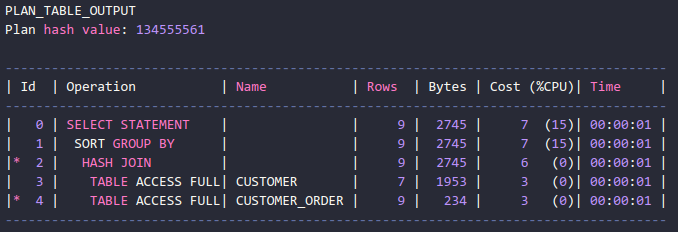
\includegraphics[scale=0.70]{img/explain_plan_without_index.png}
\end{center}
\begin{itemize}
    \item[0] SELECT - celkový select dat
    \item[1] HASH GROUP BY - vytvoření hashovací tabulky spojených pomocí řádků
    \item[2] HASH JOIN - spojení tabulek \texttt{CUSTOMER} a \texttt{CUSTOMER\_ORDER} pomocí hashovacího algoritmu
    \item[3] TABLE ACCESS FULL -  plné skenování tabulky \texttt{CUSTOMER}, která vrací 7 řádků
    \item[4] TABLE ACCESS FULL - plné skenování tabulky \texttt{CUSTOMER\_ORDER}, která vrací 9 řádků
\end{itemize}

Celkový odhad provedení je dotazu je 1 sekunda.
\newpage
\subsubsection{Provedení explain plan s indexací}
\begin{center}
    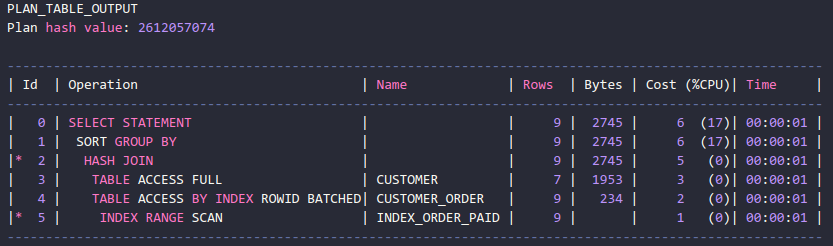
\includegraphics[scale=0.55]{img/explain_plan_with_index.png}
\end{center}

\begin{itemize}
    \item[0] SELECT - celkový select dat
    \item[1] SORT GROUP BY - seřazení výsledků podle kritérií
    \item[2] HASH JOIN - spojení tabulek \texttt{CUSTOMER} a \texttt{CUSTOMER\_ORDER} pomocí hashovacího algoritmu
    \item[3] TABLE ACCESS FULL - plné skenování tabulky \texttt{CUSTOMER}, která vrací 7 řádků
    \item[4] TABLE ACCESS BY INDEX ROWID BATCHED - přistoupení k tabulce přes index a načtou se pouze ty řádky, které jsou relevantní pro dotaz
    \item[5] INDEX RANGE SCAN - získávájí se data, která splňují podmínky dotazu pomocí indexu \texttt{index\_order\_paid}
\end{itemize}

Explain plan ukazuje že s indexací přibude jedna operace a navýší se využití CPU, ale sníží se celková cena dotazu.

\subsection{Procedures}
\begin{itemize}
    \item[1] ORDER\_STATUS\_UPDATE - získá status konkrétní objednávky a posune ji do dalšího stavu
    \item[2] ORDER\_STATUS\_LIST - vypíše všechny objednávky v zadaném stavu
\end{itemize}

\subsection{Materialized view}
Materializovaný pohled byl vytvořen pro zobrazení informací o autech a jejich řidičích.
Využili jsme: \begin{itemize}
    \item[1] CACHE - materializovaný pohled bude ukládán v cache a nebudou se opakovaně provádět dotazy na vytvoření pohledu
    \item[2] BUILD IMMEDIATE - materializovaný pohled bude vytvořen okamžitě poté, co je definice pohledu vytvořena a uložena
    \item[3] ENABLE QUERY REWRITE - umožňuje přepisovat dotazy tak, aby využívaly materializovaný pohled místo tabulek, z nichž byly vytvořeny
\end{itemize}

\subsection{With case select}
Vytvořili jsme dotaz, který se podívá na všechny objednávky a určí podle ceny jakou prioritu má objednávka. Priorita se určuje podle průměrné ceny všech objednávek.

\subsection{Privileges}
Práva byla udělena vedoucímu pekárny (xdunck01), který by měl být schopen měnit všechny údaje.

%%%%%%%%%%%%%%%%%%%%%%%%%%%%%%%%%%%%%%% 8. Závěr %%%%%%%%%%%%%%%%%%%%%%%%%%%%%%%%%%%
\section{Závěr}
Závěrem je kompletní relační databáze testována na školním serveru oracle \texttt{gort.fit.vutbr.cz} na verzi \texttt{Oracle Database 18c Enterprise Edition Release 18.0.0.0.0 - Production}
\end{document}